\section{Αισθητήρες αέρα χαμηλού κόστους και Διαδίκτυο των πραγμάτων (Internet Of Things)}


Είναι μια καθολική διαπίστωση σε μεγάλο εύρος της βιβλιογραφίας ότι ο εσωτερικός αέρας δεν έχει μελετηθεί τόσο ενδελεχώς όπως ο ατμοσφαιρικός αέρας. 
Ευτυχώς, έχει υπάρξει σημαντική αύξηση του ενδιαφέροντος των ερευνητών τα τελευταία χρόνια για τον εσωτερικό αέρα \cite{SA2022102551}.


Παραδοσιακά, η διερεύνηση της ποιότητας του εσωτερικού χώρου βασίζεται στην χρήση εργαστηριακού εξοπλισμού,
ο οποίος προσφέρει αξιόπιστα και ακριβή δεδομένα, χρήσιμα πολύ για την ακαδημαϊκή έρευνα και την δημιουργία επίσημων οδηγών και κανονισμών \cite{EUROPEANSTANDARDS2014}. 
Όμως, είναι στην πλειοψηφία των περιπτώσεων υψηλοί σε κόστος οι συγκεκριμένοι εξοπλισμοί, όποτε είναι δύσκολο και κοστοβόρο να καταγραφούν δείγματα με μεγάλο χρονικό και χωρικό εύρος.
Επίσης, καθώς αυτά τα εργαλεία κατέχονται από εργαστήριο, μετά από κάποια διαδικασία που καταγράφτηκαν ρύποι του αέρα για ένα συγκεκριμένο χώρο, 
παίρνει χρόνο να δοθούν τα αποτελέσματα πίσω στους κατοίκους των κτηρίων,
πόσο μάλλον να παρακολουθείται ο αέρας συνεχόμενα, ώστε να μπορούν να αντιδράσουν οι κάτοικοι σε ξαφνικές αλλαγές τις ποιότητας του αέρα \cite{DAI2023164858}.

Σε αυτήν την αύξηση έχει βοηθήσει σημαντικά τα τελευταία δεκαπέντε χρόνια, η μεγάλη πρόοδος της τεχνολογίας και η εμπορική διαθεσιμότητα  που έχει συντελεστεί στους αισθητήρες αέρα χαμηλού κόστους (Low Cost gas Sensors, LCS) για την παρακολούθηση της ποιότητας του αέρα.
Χάρη σε αυτούς, δίνεται έτσι σε ακόμα μεγαλύτερο εύρος ανθρώπων, χωρίς να έχουν πρόσβαση και γνώση χρήση σε εργαστηριακά εργαλεία,
η δυνατότητα συνεχής παρακολούθησης της ποιότητας το αέρα πολύ πιο εύκολα και ευέλικτα, από ότι θα μπορούσαν να πετύχουν τα παραδοσιακά μηχανήματα καταμέτρησης \cite{CHOJER2020138385},ή όργανά αναφοράς, όπως θα τα αναφέρουμε και αναφέρονται γενικά.




Δεν υπάρχει κάποιος καθολικά συμφωνημένος ορισμός για το τι μπορεί να θεωρηθεί αισθητήρας αέρα χαμηλού κόστους.
Γενικότερα, ορίζονται σαν οποιοδήποτε είδους αισθητήρα ο οποίος κοστίζει πιο φτηνά από το κόστος κατασκευής και συντήρησης 
που έχουν τα όργανα μέτρησης ποιοτήτων του αέρα που συμμορφώνονται πλήρως με τους κανονισμούς των επίσημων φορέων για το πως πρέπει να είναι αυτά τα όργανα μέτρησης \cite{CHOJER2020138385}.
Ένας πιο συγκεκριμένος ορισμός που θα μπορούσε να δοθεί, είναι ότι οι αισθητήρες αέρα χαμηλού κόστους είναι τεχνολογίες που υπόσχονται μια επαναστατική πρόοδο στην παρακολούθηση της ποιότητας του αέρα,
μέσω τεράστιων αυξήσεων στη χωρική και χρονική ανάλυση των δεδομένων, παρέχοντας έτσι απαντήσεις σε επιστημονικά ερωτήματα και εφαρμογές. \cite{MORAWSKA2018286}.



Όταν στην βιβλιογραφία γίνεται αναφορά για αισθητήρες φτηνού κόστους, 
υπονοούνται ταυτόχρονα και οι μεμονωμένοι αισθητήρες που παράγονται από κατασκευαστές αρχικού εξοπλισμού (Original equipment manufacturer, OEM),
αλλά και τα συστήματα αισθητήρων (System sensors), τα οποία περιλαμβάνουν τους αισθητήρες OEM μαζί με κουτί προστασίας, 
σύστημα δειγματοληψίας, σύστημα τροφοδοσίας, ηλεκτρονικό υλικό και λογισμικό για απόκτηση δεδομένων, μετατροπή από αναλογικό σε ψηφιακό σήμα, επεξεργασία δεδομένων και μεταφορά δεδομένων \cite{atmos10090506}.

Από την πλευρά του χρήστη, τα συστημάτων αισθητήρων είναι έτοιμα προς χρήση συστήματα, ενώ οι χρήστες των αισθητήρων OEM χρειάζεται να προσθέσουν εξαρτήματα υλικού και λογισμικού για προστασία από μετεωρολογικές συνθήκες, αποθήκευση δεδομένων, αποστολή δεδομένων, 
διαλειτουργικότητα των δεδομένων και βαθμονόμηση (calibration) των αισθητήρων.
Η breakout πλακέτα, που είναι μία ειδική κατηγορία πλακετών τυπωμένου κυκλώματος που δίνει ρεύμα στους αισθητήρες και εύκολες διασυνδέσεις με μικροελεκτές και άλλες ηλεκτρονικές συσκευές \cite{JLCPCB2024},
αντιμετωπίζεται πάντα σαν ένα αναπόσπαστο κομμάτι των LCS, αλλά μπορεί να είναι από την ίδια ή διαφορετική εταιρία.

Η βαθμονόμηση είναι η διαδικασία ρύθμισης ενός οργάνου μέτρησης, για να εξασφαλιστεί ότι το αποτέλεσμα που δίνει το όργανο αυτό για κάποιο δείγμα είναι σε ένα αποδεκτό σωστό εύρος τιμών \cite{Kotsonis2024}.
Στις περιπτώσεις των αισθητήρων φτηνού κόστους (LCS), είναι η σύγκριση των μετρήσεων του με έναν αισθητήρα που είναι όργανο αναφοράς και η μετατροπή των εξόδων του, ώστε να συμφωνεί με τα αποτελέσματα του οργάνου αναφοράς.

Η μέθοδος που χρησιμοποιείται για την βαθμονόμηση των LCS θεωρείται γενικά από την πλειονότητα των κατασκευαστών LCS ως εμπιστευτική πληροφορία.
Ελάχιστες πληροφορίες είναι διαθέσιμες σχετικά με τη βαθμονόμηση των LCS που έχουν την λειτουργία τους σε κλειστό κώδικα . 
Αντιθέτως, αρκετές πληροφορίες και μελέτες υπάρχουν για την βαθμονόμηση των LCS ανοικτού κώδικα, τόσο σε εργαστηριακές συνθήκες, όσο  πραγματικά περιβάλλοντα. 

Η βαθμονόμηση των LCS ανοικτού κώδικα συνίσταται στον καθορισμό ενός μαθηματικού μοντέλου που περιγράφει τη σχέση μεταξύ των δεδομένων του LCS και των μετρήσεων αναφοράς.
Ωστόσο, οι περισσότερες διαδικασίες βαθμονόμησης πραγματοποιήθηκαν κατά τη διάρκεια δοκιμών, ενώ μόνο ένας περιορισμένος αριθμός πειραμάτων βαθμονόμησης σε εργαστήριο βρέθηκε \cite{atmos10090506}.
Γενικά, η πλειοψηφία των LCS έχουν όλο ή μερικό κομμάτι της λειτουργίας τους σαν εμπιστευτική πληροφορία,οπότε είναι δύσκολο να έχουμε πλήρη γνώση πως λειτουργούν,
ακόμα και σε σημαντικές διεργασίες όπως είναι η βαθμονόμηση.
Υ

Ενώ οι LCS προσφέρουν παρά πολλές δυνατότητες και έχει βρεθεί να δίνουν ικανοποιητικά αποτελέσματα, δεν είναι πλήρως αξιόπιστοι.
Πέρα από την ακρίβεια των μετρικών τους που δεν είναι τόσο καλή  στην πραγματικότητα είναι ευαισθησία των LCS σε άλλους ρύπους από αυτούς που υποτίθεται ότι όντως μετράει (cross-sensitivity), 
την σταδιακή απόκλιση των εξόδου τους από την πραγματική τιμή κατά την διάρκεια λειτουργίας τους μες στο χρόνο (sensor drift).
Το sensor drift είναι κάτι που υπάρχει στους αισθητήρες γενικά, αλλά είναι πιο έντονο στους LCS, που αρχίζει να επιδράει μέσα σε κάποιες μήνες.
Ακόμα, υπάρχει έντονη επιρροή περιβαλλοντικών παραμέτρων, όπως υγρασία και θερμοκρασία.

Αυτό που έχει αναδειχθεί από έρευνες είναι ότι οι LCS μπορούν να χρησιμοποιηθούν για ποιητική παρακολούθηση του αέρα, για να μπορούν οι χρήστες να κρίνουν αν ο αέρας είναι σε υψηλά επίπεδα ρύπανσης ή όχι,
ώστε να αντιμετωπίσουν το πρόβλημα ανάλογα, όπως με εξαερισμό.
Μπορούν να χρησιμοποιηθούν και για ποσοτική παρακολούθηση των ρύπων του αέρα, αν έχει υπάρξει διαδικασία βαθμονόμησης με όργανο αναφοράς.
Η βαθμονόμηση συνιστάται να γίνεται στις πραγματικές συνθήκες περιβάλλοντος που θα δουλέψει ο αισθητήρας και όχι μόνο σε εργαστήριο.
Για μέγιστη ακρίβεια, επιθημειτή είναι η βαθμονόμηση σε συχνότητα κάποιων μηνών, για να αντιμετωπιστεί το πρόβλημα της απόκλισης του αισθητήρα ανά το χρόνο.

Δυστυχώς,λόγω της έλλειψης κοινών προτύπων για το πως θα γίνει η βαθμονόμηση και πως θα έλεγχθει η απόδοση των LCS σε κάθε ερεύνα,
δεν είναι εύκολα να αξιολογηθεί πόσο έμπιστα τα δεδομένα των LCS είναι σε σχέση με τα καθιερωμένα όργανα αναφοράς,
ωστέ να μπορούν τα δεδομένα τους να χρησιμοποιηθούν σε ερευνητικές μελετές \cite{SA2022102551}, \cite{CHOJER2020138385}.

Μια ενδελεχής ανάλυση των LCS γίνεται από τον Goncalo Marques στην ανασκόπηση \cite{Garcia2022},ο οποίος αποτελεί τον ερευνητή με τις περισσότερες δημοσιεύσεις στον τομέα της παρακολούθησης του εσωτερικού αέρα,
χρησιμοποιώντας LCS και Διαδίκτυο των πραγμάτων (Internet Of Things) \cite{Tan2024}.
Ενώ διαβάστηκαν πολλές ανασκοπήσεις και έρευνες στον τομέα των LCS, η παραπάνω ανασκόπηση θεωρούμε ότι καλύπτει πλήρως τα θετικά και αρνητικά των LCS, όπως και λεπτομέρειες της λειτουργίας και της χρήση τους.

\subsection{Είδη LCS}

Οι παρακάτω κατηγορίες και περιγραφές έχουν παρθεί από το συμπληρωματικό υλικό της έρευνας των \cite{Garcia2022}:
\subsubsection{Ηλεκτροχημικοί αισθητήρες (Electrochemical sensors ,EC)}

Οι ηλεκτροχημικοί αισθητήρες μετατρέπουν την επίδραση μιας ηλεκτροχημικής αλληλεπίδρασης μεταξύ του επιλεγμένου για μέτρηση  αερίου και του ηλεκτροδίου σε ηλεκτρικό σήμα, το οποίο είναι ανάλογο της συγκέντρωσης του αερίου [1, 2]. Οι αισθητήρες αυτοί περιλαμβάνουν ένα στοιχείο που περιέχει ηλεκτρολύτη καθώς και δύο ή τρία ηλεκτρόδια, και όταν ο αισθητήρας έρχεται σε επαφή με το επιλεγμένο αέριο, πραγματοποιείται οξείδωση ή μείωση, παράγοντας ένα μετρήσιμο ρεύμα μεταξύ των ηλεκτροδίων εργασίας και αντίθεσης. Οι περισσότεροι LCS διαθέτουν ένα τρίτο αναφορικ» ηλεκτρόδιο προκειμένου να βελτιώσουν τη γραμμικότητα και την ευαισθησία [2, 3]. Οι αισθητήρες αυτοί μπορεί να είναι ευάλωτοι σε παρεμβολές από περιβαλλοντικές παραμέτρους και από άλλες χημικές ενώσεις [4].


\subsubsection{Ημιαγωγοί Μεταλλικού Οξειδίου (Metal Oxide Semiconductors,MOS)}

Η αρχή λειτουργίας των αισθητήρων ημιαγωγικού μεταλλικού οξειδίου 
βασίζεται στην απορρόφηση οξυγόνου σε υψηλές θερμοκρασίες στην επιφάνεια των οξειδίων μετάλλων,
 παγιδεύοντας έτσι ηλεκτρόνια από το εσωτερικού του υλικού, αυξάνοντας ή μειώνοντας την αντίσταση του αισθητήρα για υλικά τύπου n ή p,
  αντίστοιχα. Στον αέρα, σε θερμοκρασίες μεταξύ $150^\circ \mathrm{C}$ και $400^\circ \mathrm{C}$, το οξυγόνο απορροφάται στην επιφάνεια.
   Το επιλεγμένο προς μέτρηση αέριο  αντιδρά με το προσροφημένο οξυγόνο ή άμεσα με το οξείδιο, προκαλώντας μεταβολή της αντίστασης του αισθητήρα, η οποία ανιχνεύεται ως σήμα του αισθητήρα και σχετίζεται με τη συγκέντρωση του  επιλεγμένο προς μέτρηση αερίου [5, 6].
    Οι αισθητήρες MOS αποτελούν τη χαμηλή κόστους λύση για την παρακολούθηση της ποιότητας του αέρα, ωστόσο παρουσιάζουν σημαντικές προκλήσεις στην ποσοτικοποίηση, όπως διασταυρούμενες ευαισθησίες (cross-sensitivity)  και εξάρτηση από την σχετική υγρασία και τη θερμοκρασία [7].

\subsubsection{Μη Διασπειρόμενο Υπέρυθρος,(Non-Dispersive InfraRed ,NDIR)}

Αυτός ο τύπος αισθητήρα βασίζεται στις οπτικές ιδιότητες του επιλεγμένου προς μέτρηση αερίου, δηλαδή στα μήκη κύματος στα οποία το αέριο απορροφά το φως. Ο αισθητήρας αποτελείται από μια πολυχρωματική πηγή φωτός, συνήθως μια λυχνία ή LED, ένα κυψελίδιο αερίου, ένα φίλτρο ζώνης (band-pass) για τον περιορισμό του εισερχόμενου φωτός στη συγκεκριμένη φασματική ζώνη απορρόφησης του αναλυτή, και τον ανιχνευτή. Πολλά αέρια ρύπων είναι ενεργά στο υπέρυθρο (IR) φάσμα (π.χ. CO, CO\textsubscript{2}, SO\textsubscript{2}, NO\textsubscript{x}, N\textsubscript{2}O, N\textsubscript{3}, HCl, HF και CH\textsubscript{4}), και μπορούν δυνητικά να παρακολουθηθούν με αυτή τη μέθοδο. Η ποσοτικοποίηση στις μετρήσεις NDIR βασίζεται στον νόμο απορρόφησης Beer-Lambert [9, 10].

\subsubsection{Ανιχνευτής Φωτοϊονισμού (Photoionization detectors, ID)}

Η λειτουργία τους βασίζεται στην απορρόφηση φωτονίων από μια πηγή φωτοεκκένωσης από ένα μόριο του στοχευόμενου αερίου, οδηγώντας στο σχηματισμό ενός διεγερμένου μορίου, δηλαδή φωτοϊόντων. Όταν η ενέργεια των φωτονίων hν υπερβαίνει την ενέργεια ιονισμού του μορίου, εκπέμπεται ένα ηλεκτρόνιο και σχηματίζεται ένα κατιόν, το οποίο κατευθύνεται προς ένα ηλεκτρόδιο, παράγοντας ηλεκτρικό ρεύμα που εξαρτάται από τον αριθμό των διεγερμένων μορίων και, συνεπώς, από τη συγκέντρωση του ανιχνευόμενου αερίου [8]. Στους PID χρησιμοποιούνται διάφοροι τύποι λυχνιών. Οι αισθητήρες PID εμφανίζουν σύντομο χρόνο απόκρισης (λίγα δευτερόλεπτα) και δεν είναι ειδικοί για κάποιο συγκεκριμένο αναλυτή, αλλά παρουσιάζουν υψηλή ευαισθησία σε αλκοόλες, αρωματικές ενώσεις, αλδεΰδες και κετόνες, λιπαρά οξέα και πολυκυκλικούς αρωματικούς υδρογονάνθρακες (PAH), με τους τελευταίους να ανιχνεύονται ακόμη και σε χαμηλότερες συγκεντρώσεις σε σχέση με αυτές που μπορούν να επιτευχθούν με αισθητήρες NDIR [9].



\subsubsection{Διασκορπισμός φωτός (Light Scattering)}

Στην περίπτωση των σωματιδίων αιωρούμενης ύλης PM, η βασική αρχή ανίχνευσης στηρίζεται στη σκέδαση, ή διασκορπισμό φωτός, κατά την οποία ο αέρας από το περιβάλλον που παρακολουθείται οδηγείται μέσα στο περίβλημα του αισθητήρα, όπου χρησιμοποιείται μια πηγή φωτός σε συνδυασμό με φωτοδίοδο. Τα σωματίδια προκαλούν σήμα σκέδασης φωτός, το οποίο συνήθως μετατρέπεται σε αναλογικό σήμα τάσης ή σήμα διαμόρφωσης πλάτους παλμών (pulse width modulation), που χρησιμοποιείται για την αναπαράσταση των μετρούμενων συνθηκών, όπως πλήθος παλμών, ύψος ή διάρκεια παλμών. Το σήμα αυτό μπορεί να αναλυθεί ως προς τη συχνότητα των παλμών, εκτιμώντας έτσι τον αριθμό των σωματιδίων, και ως προς το αντίστοιχο ύψος των παλμών, παρέχοντας εκτίμηση του μεγέθους των σωματιδίων. Εναλλακτικά, η συνολική ένταση του σκορπισμένου φωτός μπορεί να χρησιμοποιηθεί για την εκτίμηση ενός συνόλου σωματιδίων [11]. Η μέθοδος αυτή ονομάζεται νεφελομετρική σκέδαση.

\subsubsection{Θάλαμοι ιονισμού (Ionization Chambers)}

θαλάμη ιονισμού αποτελεί ενεργό στοιχείο αισθητήρα που χρησιμοποιείται συχνά για την ανίχνευση ιοντίζουσας ακτινοβολίας. Στην περίπτωση του ραδονίου, χρησιμοποιούνται για την ανίχνευση σωματιδίων α και μπορούν να λειτουργούν για αξιολόγηση βραχυχρόνιας ή μακροχρόνιας έκθεσης. Όταν ένα φορτισμένο σωματίδιο διέρχεται από τη θαλάμη παρουσία ιοντίζουσας ακτινοβολίας, παράγονται ζεύγη ηλεκτρονίου-ιόντος, τα οποία επιταχύνονται λόγω του εφαρμοζόμενου ηλεκτρικού πεδίου μέχρι να συγκρουστούν με τα ηλεκτρόδια [12]. Στη συνέχεια, ένα ηλεκτρονικό κύκλωμα παράγει έναν ηλεκτρικό παλμό ανά σύγκρουση, οι οποίοι στη συνέχεια καταμετρώνται για συγκεκριμένα χρονικά διαστήματα [13]. Συνήθως, οι LCS για το ραδόνιο χρησιμοποιούν θαλάμες ιονισμού [14, 15], λόγω της απλής κατασκευής τους, της προσιτής τιμής και της ικανοποιητικής ακρίβειας.

\subsubsection{Φασματομετρία άλφα (Alpha Spectrometry )}

Η άλφα-φασματομετρία μπορεί να χρησιμοποιηθεί για την ταυτοποίηση και ποσοτικοποίηση των σωματιδίων α που εκπέμπονται κατά τη διαδικασία διάσπασης ραδιονουκλεϊδίων, όπως το ραδόνιο. Στη διαδικασία αυτή, η ιοντίζουσα ακτινοβολία μπορεί να ανιχνευθεί μέσω αλφα-φασματομετρίας [16, 17]. Συνήθως, οι υλοποιήσεις χαμηλού κόστους της αλφα-φασματομετρίας βασίζονται σε φωτοδιόδους PIN, ευαίσθητες σε σωματίδια α [18], οι οποίες μπορούν να υλοποιηθούν χρησιμοποιώντας εμπορικά διαθέσιμα εξαρτήματα [19].


\subsection{Internet Of Things}

Για την συνεχή παρακολούθηση του αέρα με έναν ή πολλούς αισθητήρες, το δίκτυο που σχηματίζεται μεταξύ της συσκευή που διαχειρίζεται τον αισθητήρα και της συσκευής που έχουμε αποφασίσει να συλλέξει 
τα δεδομένα που παίρνουμε από όλους τους αισθητήρες, ονομάζεται  το διαδίκτυο των πραγμάτων (Internet of Things,IoT)


%γράψε περισσότερα για τους αισθητήρες, τις κατηγορίες τους και τα προβλήματα που υπάρχουν
Το Internet of Thing ορίζεται έως ένα δίκτυο σχετιζόμενων συσκευών που συνδέονται και εναλλάσσουν δεδομένα μεταξύ τους, σε gateaway συσκευή ή και στο ίντερνετ σε κάποιο cloud.
Έχουν ενσωματωμένο λογισμικό, κάποιου είδος αισθητήρα ή πολλούς αισθητήρες μαζί και μπορεί να περιέχει και μπορεί να περιλαμβάνει μηχανικές και ψηφιακές μηχανές, καθώς και καταναλωτικά αντικείμενα.
 Αυτές οι συσκευές μπορεί να είναι καθημερινές οικιακά αντικείμεα έως και περίπλοκα μηχανίματα που χρησιμοποιούνται στην βιομηχανία. \cite{TechTarget2025}.


\begin{figure}[!htbp]
    \centering
    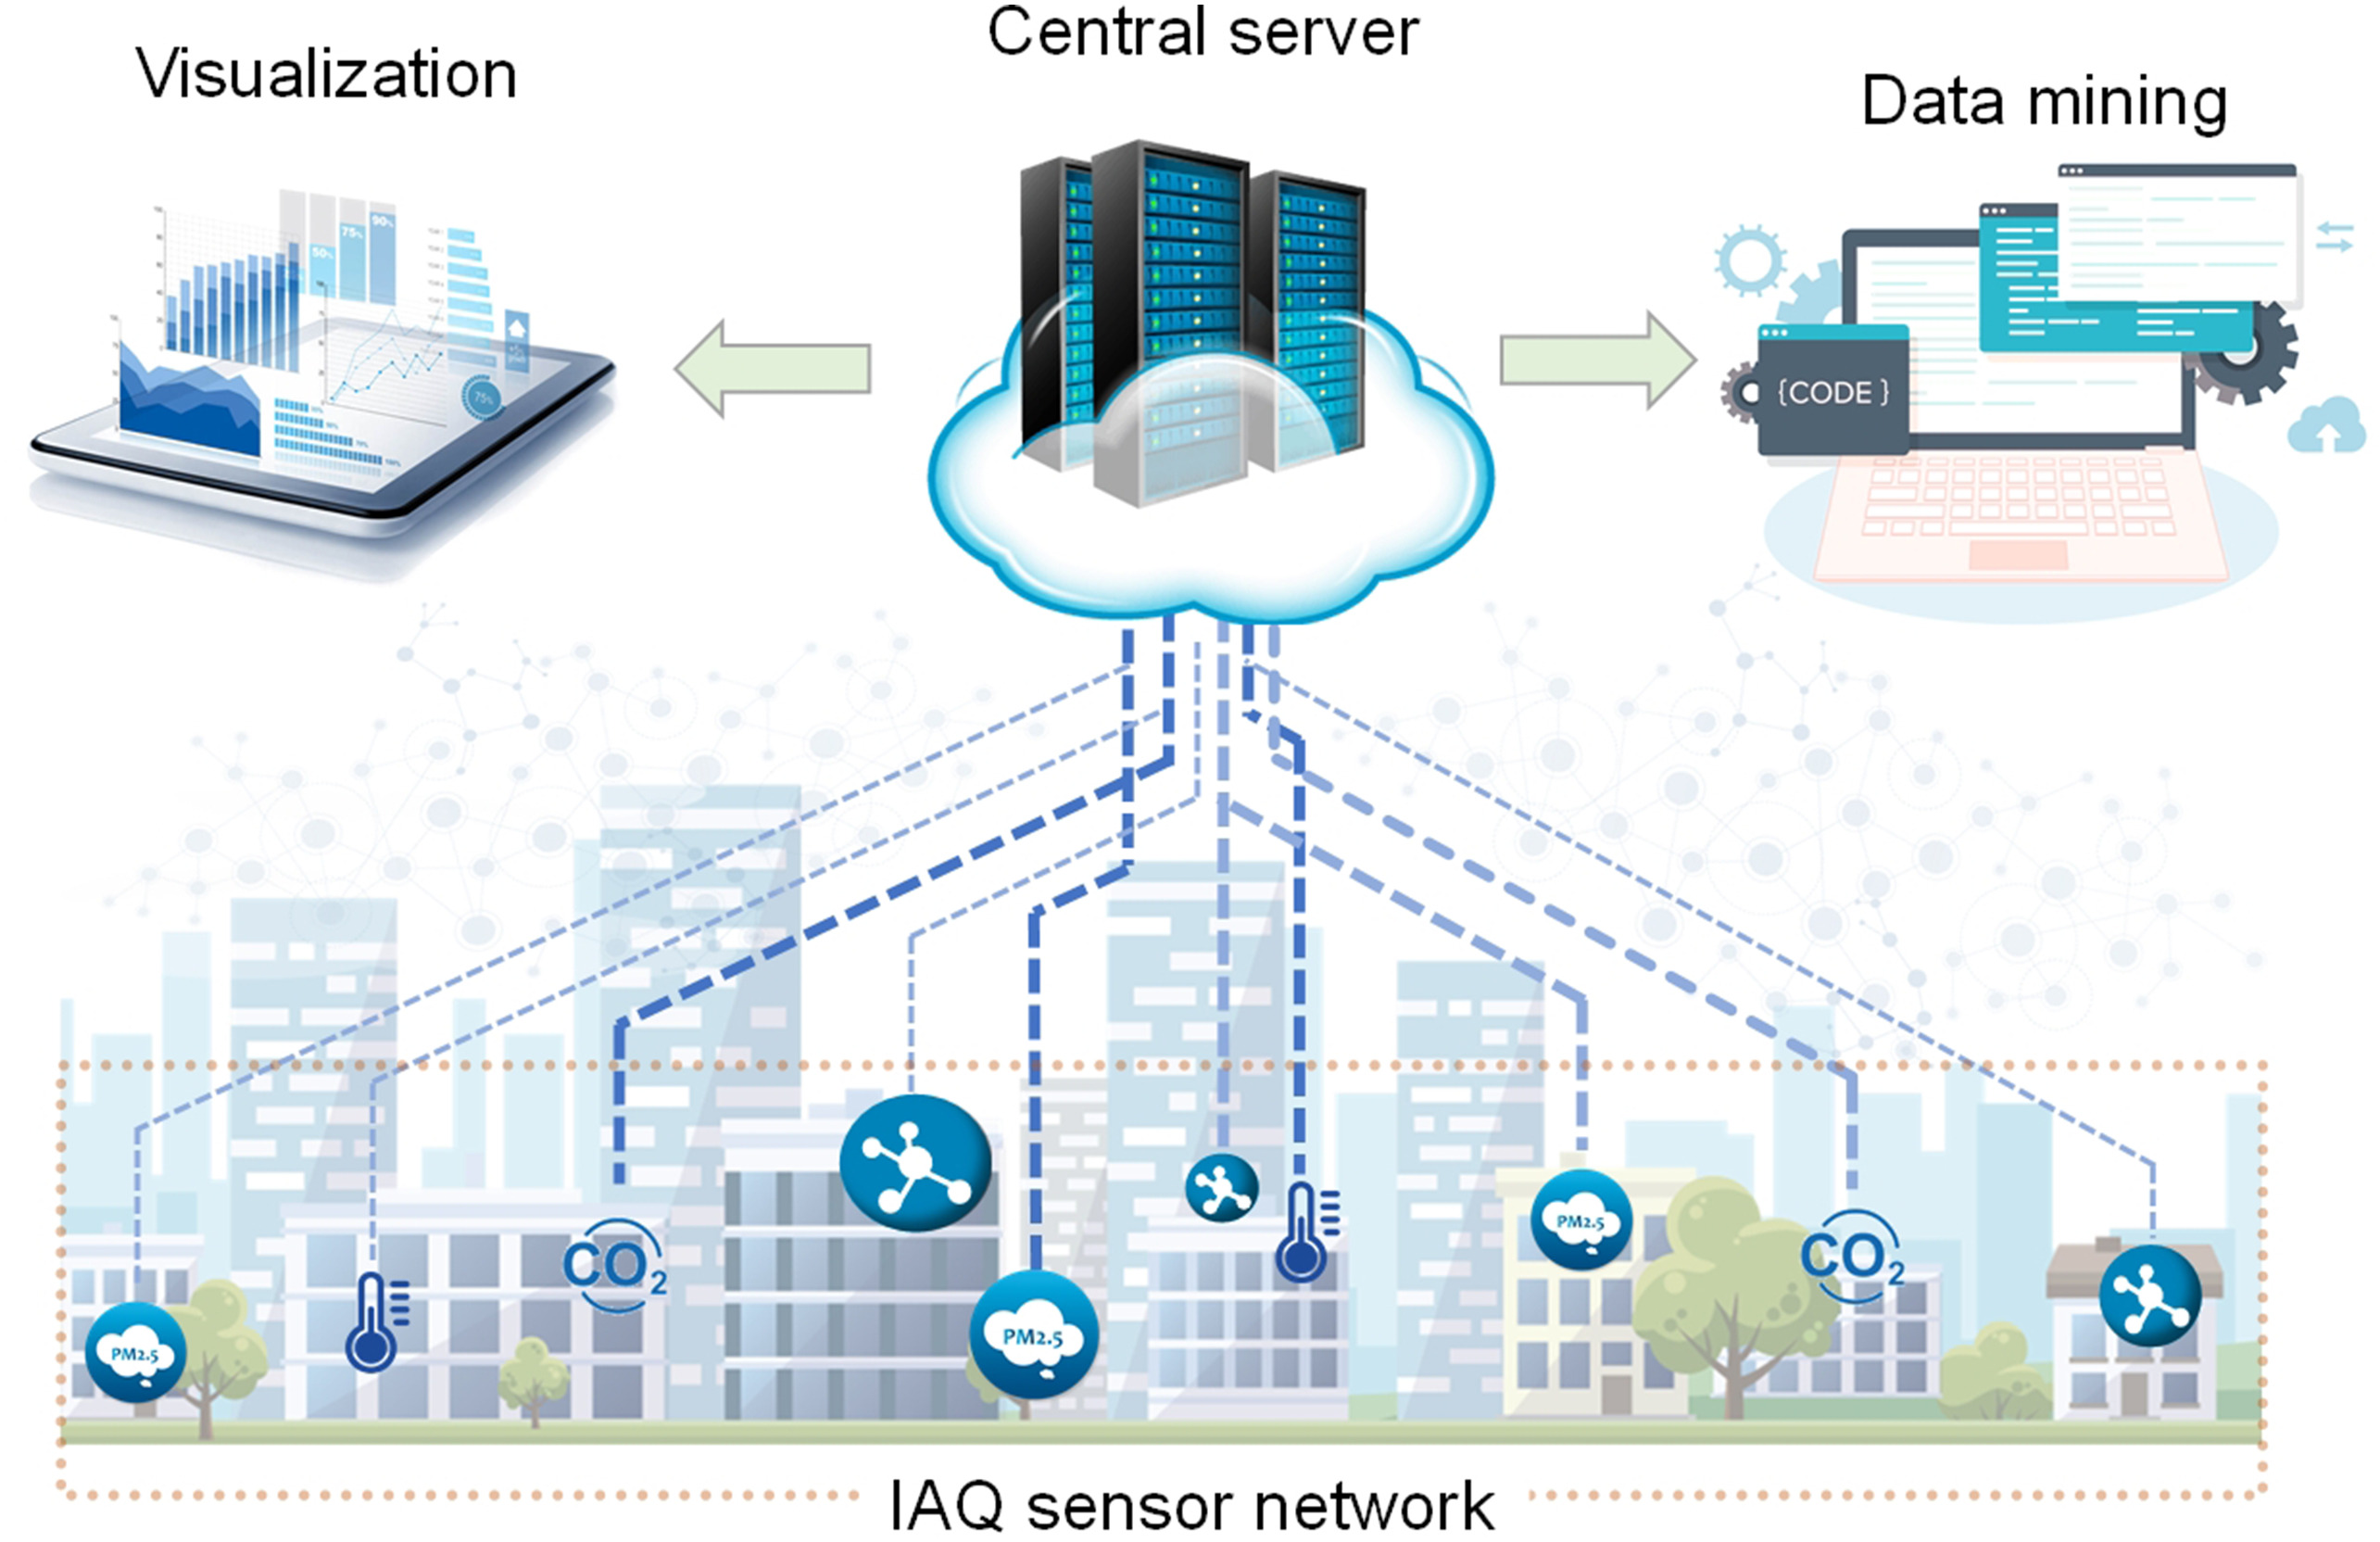
\includegraphics[width=0.8\textwidth]{εικόνες/IoT IAQ image.jpg}
    \caption{Διάγραμμα με συνοπτική περιγραφή του IoT στο κομμάτι της ποιότητας εσωτερικού αέρα\cite{DAI2023164858}}
    \label{fig:IoTIAQ}
\end{figure}


Το IoT έχει επιφέρει σημαντικές εξελίξεις στις τεχνολογίες αισθητήρων και στον έλεγχο σε πολλούς τομείς,
στις μεταφορές, την ενέργεια και τα έξυπνα κτήρια (smart buildings). 
Στον τομέα της συνεχής παρακολούθησης της ποιότητας του αέρα, έχουν φτιαχτεί πολλές πλατφόρμες IoT,
ειδικά από το 2015 και μετά, 
με κάποιες από αυτές τις πλατφόρμες να έχουν χρησιμοποιήσει data driven μεθόδους για την πρόβλεψη μελλοντικών τιμών και της εξαγωγή γνώσεων για το ποιότητα του εσωτερικού αέρα. \cite{DAI2023164858}

\FloatBarrier